The first thing we want to answer in this paper is about browser features, feature trends, and feature lifespan. We extracted every feature existing in all of the browser versions in our test platform using the collection system discussed in section 2.1.1. After extracting feature information for all of the browsers, we parsed the reports to generated useful information about them. We categorize browser features into 3 different categories.

\begin{itemize}
    \item Permanently Added: Features that are added to a specific version and exist in every other version that is released after the first version. These features should appear in at least two versions to be considered into this category.
    \item Permanently Removed: Features that existed in older versions but were removed since introducing a specific version and never appeared in newer versions again. These features should not appear in at least two latest versions to be considered permanently removed.
    \item Experimental: These are features that are being added and removed every now and then. These features do not follow a straight trend and are being tested by vendors. Features that are not included in the above categories will be considered experimental.
\end{itemize}

Before starting our main analysis, we take a look at these feature categories by comparing feature category sizes between Firefox and Chrome. We see that Chrome has 9482 permanently added features, 711 permanently removed, and 3397 experimental features. On the other hand, Firefox has 6237 permanently added, 809 permanently removed, and 152 experimental features. As we see, Firefox tends to be more stable by adding less experimental features. Also, they add significantly less features compared to Chrome but they are also removing more features permanently. In figure A and B, we illustrate the portion of each feature category among the others.

\begin{figure}[ht]
    \centering
    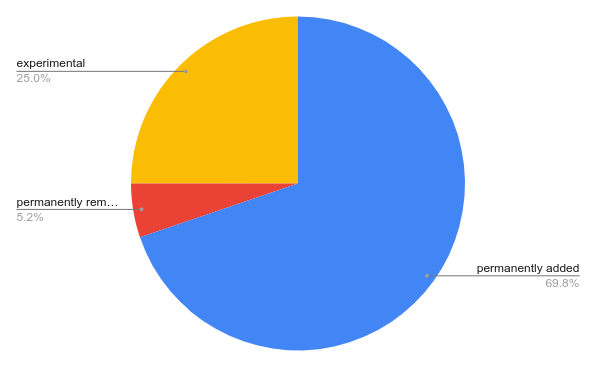
\includegraphics[width=\columnwidth]{figures/Chrome-feature-categories.png}
    \caption{Chrome feature categories. We see that permanently added features have the major portion, then we have experimental features, and the permanently removed features have the least share among other categories.}
    \label{fig:chrome-categories}
\end{figure}

\begin{figure}[ht]
    \centering
    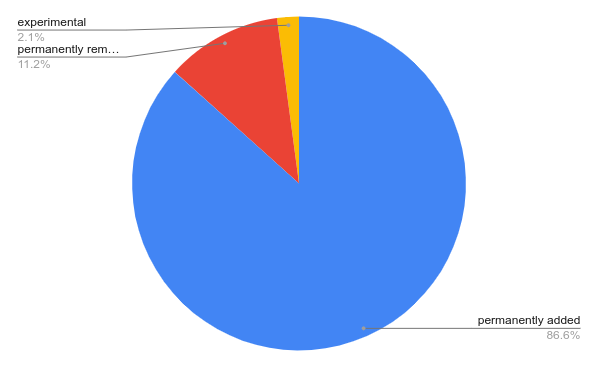
\includegraphics[width=\columnwidth]{figures/Firefox-feature-categories.png}
    \caption{Firefox feature categories. We see that permanently added features have the major portion, then we have permanently removed features, and the experimental features have the least share among other categories.}
    \label{fig:firefox-categories}
\end{figure}

We also take a look at the common feature set between Firefox and Chrome. The total number of features that these browsers have had since the beginning is 15945 features. There exists only 4843 common features among them which is approximately \%30 of the total. So we figure out that the feature set between Firefox and Chrome highly varies and they are not much similar. Although both of these browsers may have the same functionality for specific purposes, they might have different APIs which means we categorize these two APIs as different features. One of these APIs may face a specific vulnerability while the other one is invulnerable to that specific CVE.

After gathering all the feature information about every browser and generating a feature set for each browser version, by comparing the feature set between different versions we find out how many features are added and removed from each version. Our results show that Chrome is adding and removing many more features compared to Firefox. But Firefox removes a bigger portion of its features in each version and tries to keep its feature number more steady. Figure 1 and Figure 2 show how this trend looks like among these browsers.

\begin{figure}[ht]
    \centering
    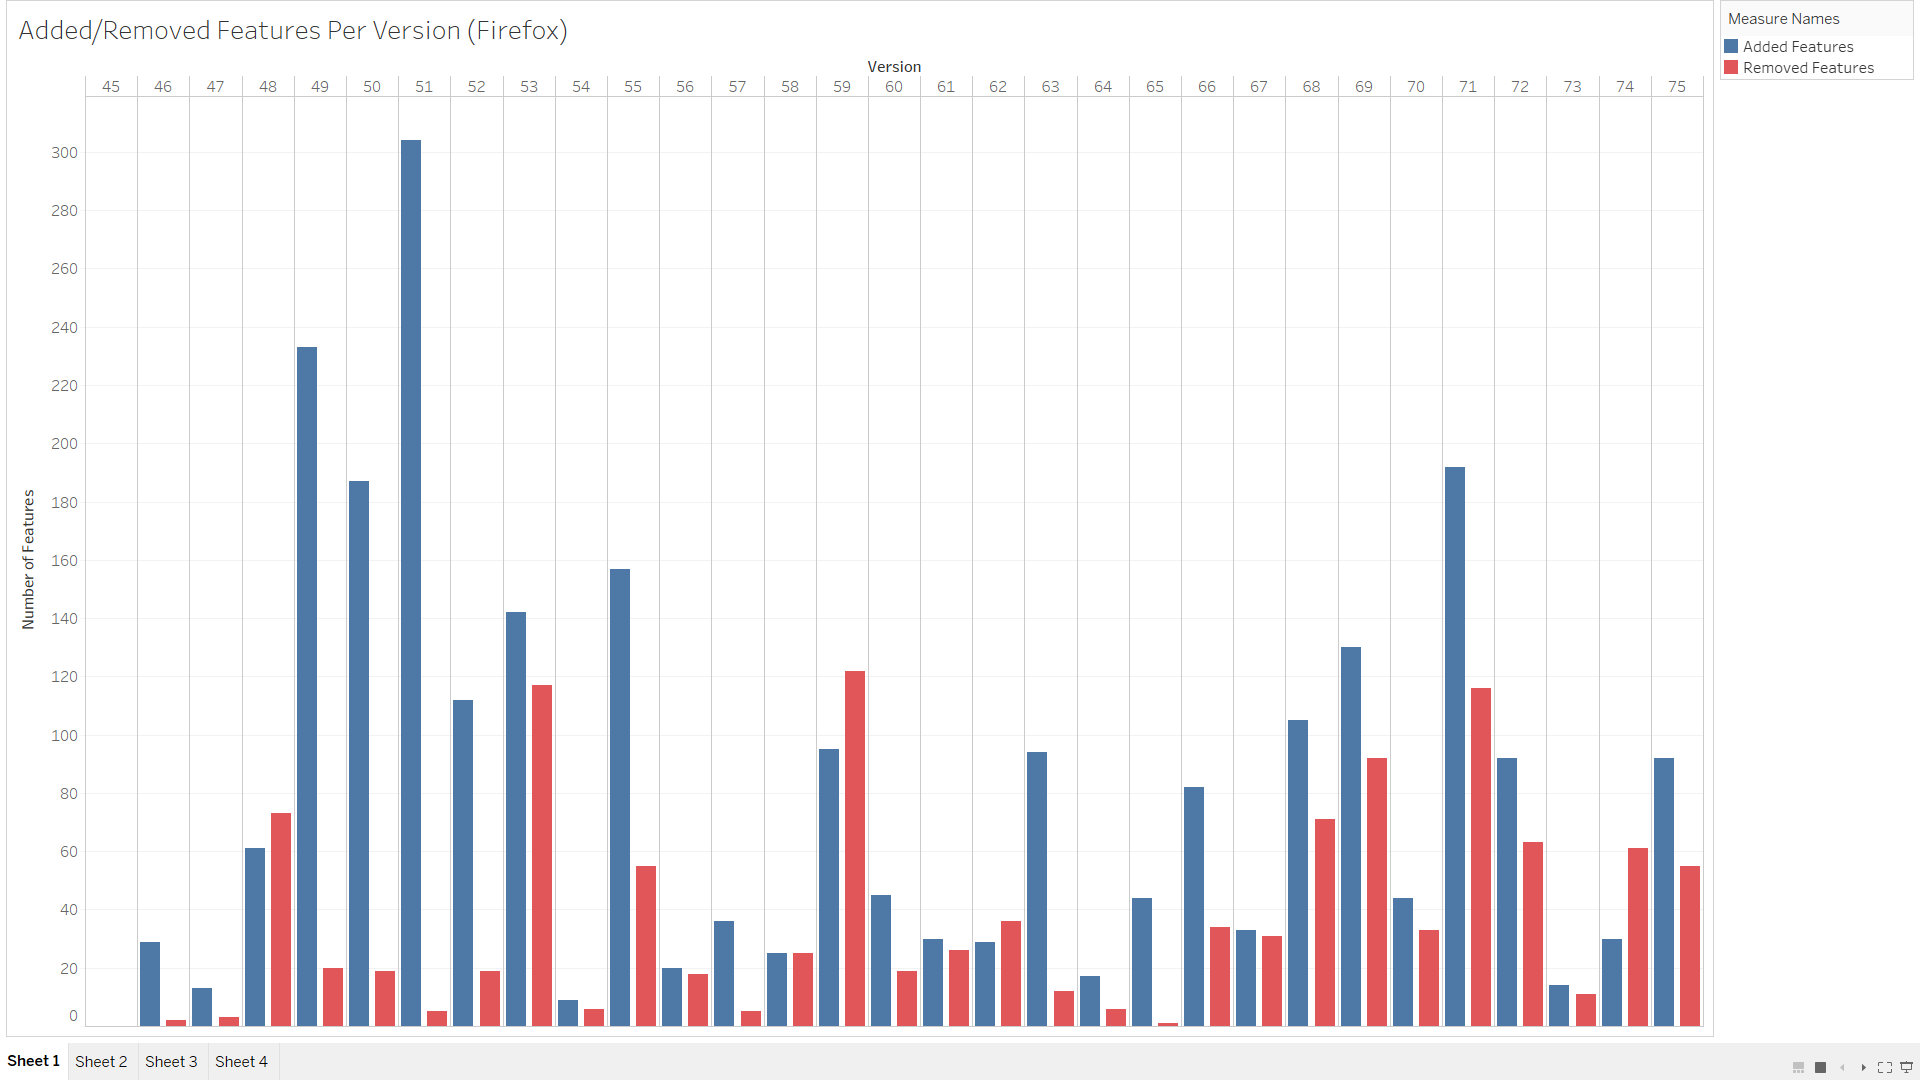
\includegraphics[width=\columnwidth]{figures/Firefox-add-remove.png}
    \caption{Feature Introduction and removal in Firefox. Red bars represent the removed features and the blue bars represent added features.}
    \label{fig:times_bar}
\end{figure}

\begin{figure}[ht]
    \centering
    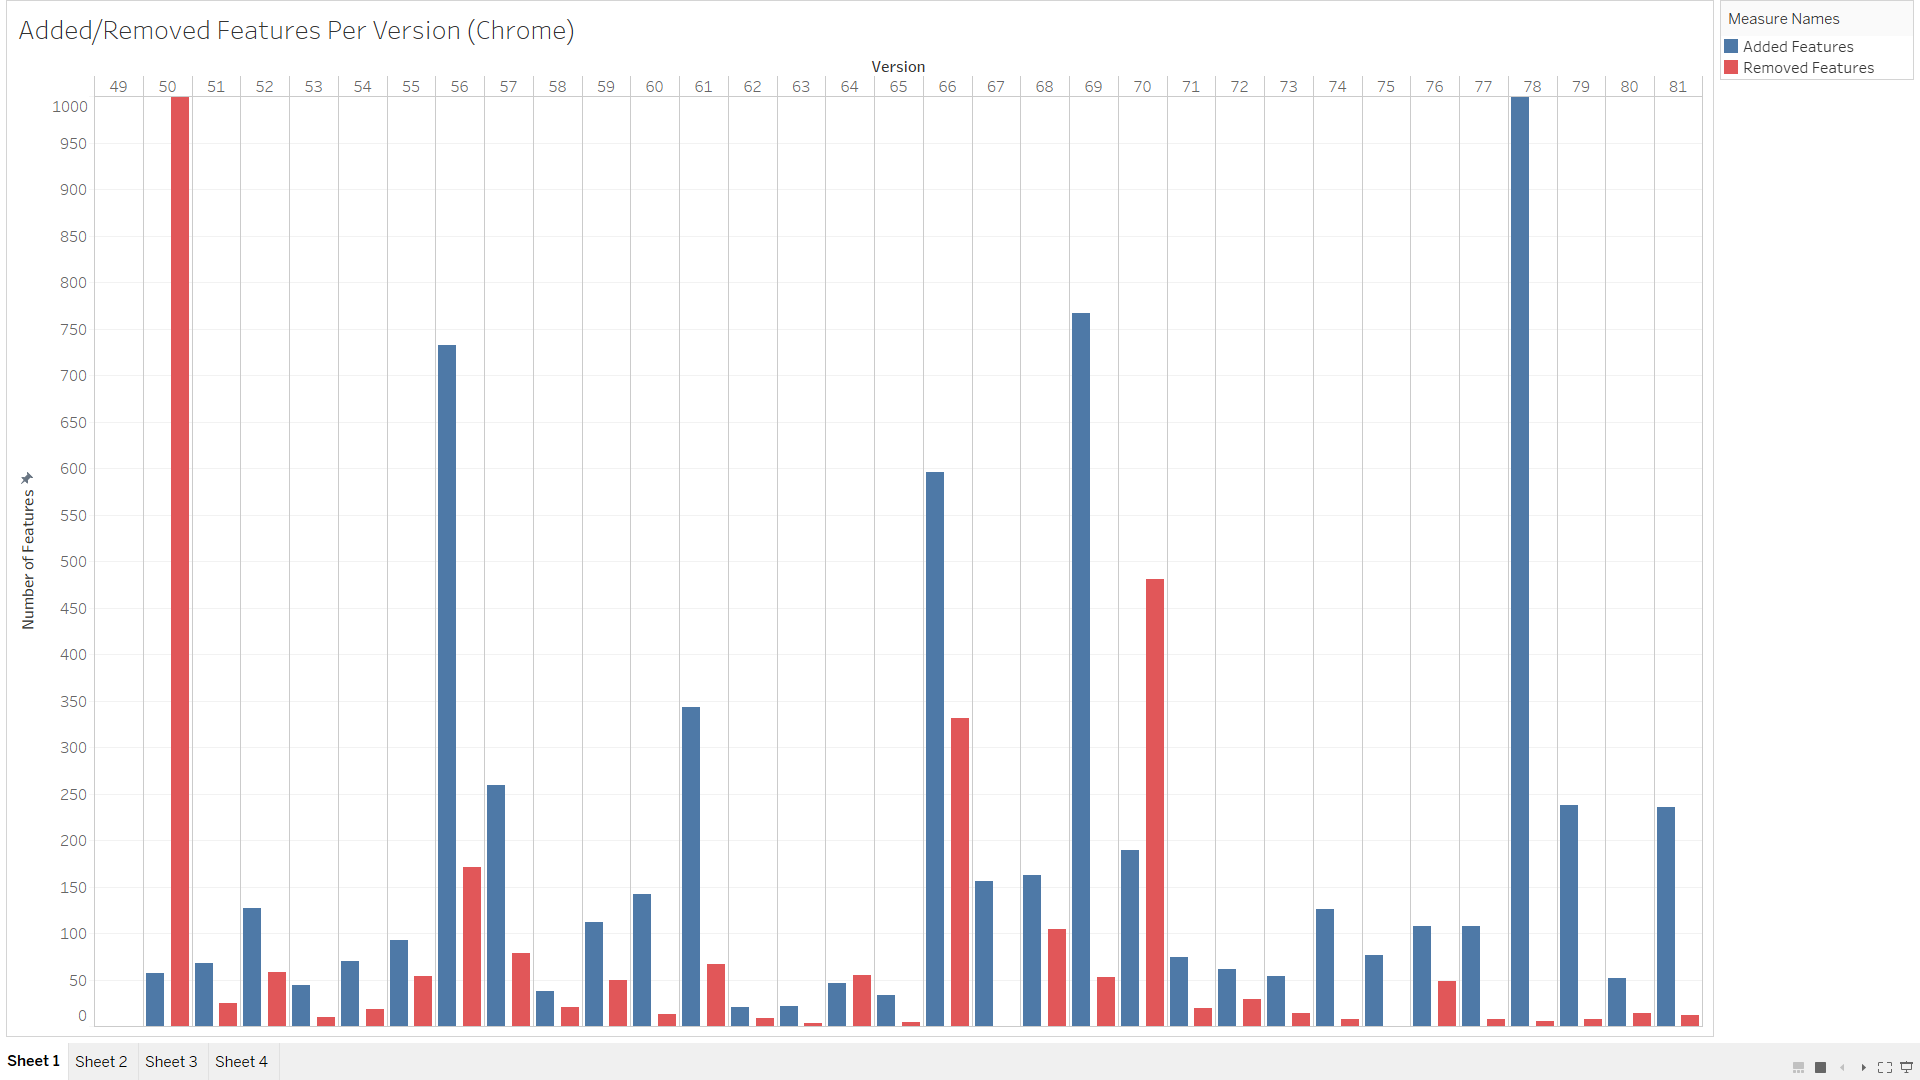
\includegraphics[width=\columnwidth]{figures/Chrome-add-remove.png}
    \caption{Feature Introduction and removal in Chrome. Red bars represent the removed features and the blue bars represent added features.}
    \label{fig:times_bar}
\end{figure}

By using the extracted data for the previous part, we tried to compare feature trends in Chrome and Firefox. We see that Chrome is adding many more features to its browsers comparing to Firefox. Firefox tries to keep the number of its features more steady. They try to remove a bigger portion of their feature set in each version. We cannot say one of them is following the other one in terms of feature introduction and removal.

\begin{figure}[ht]
    \centering
    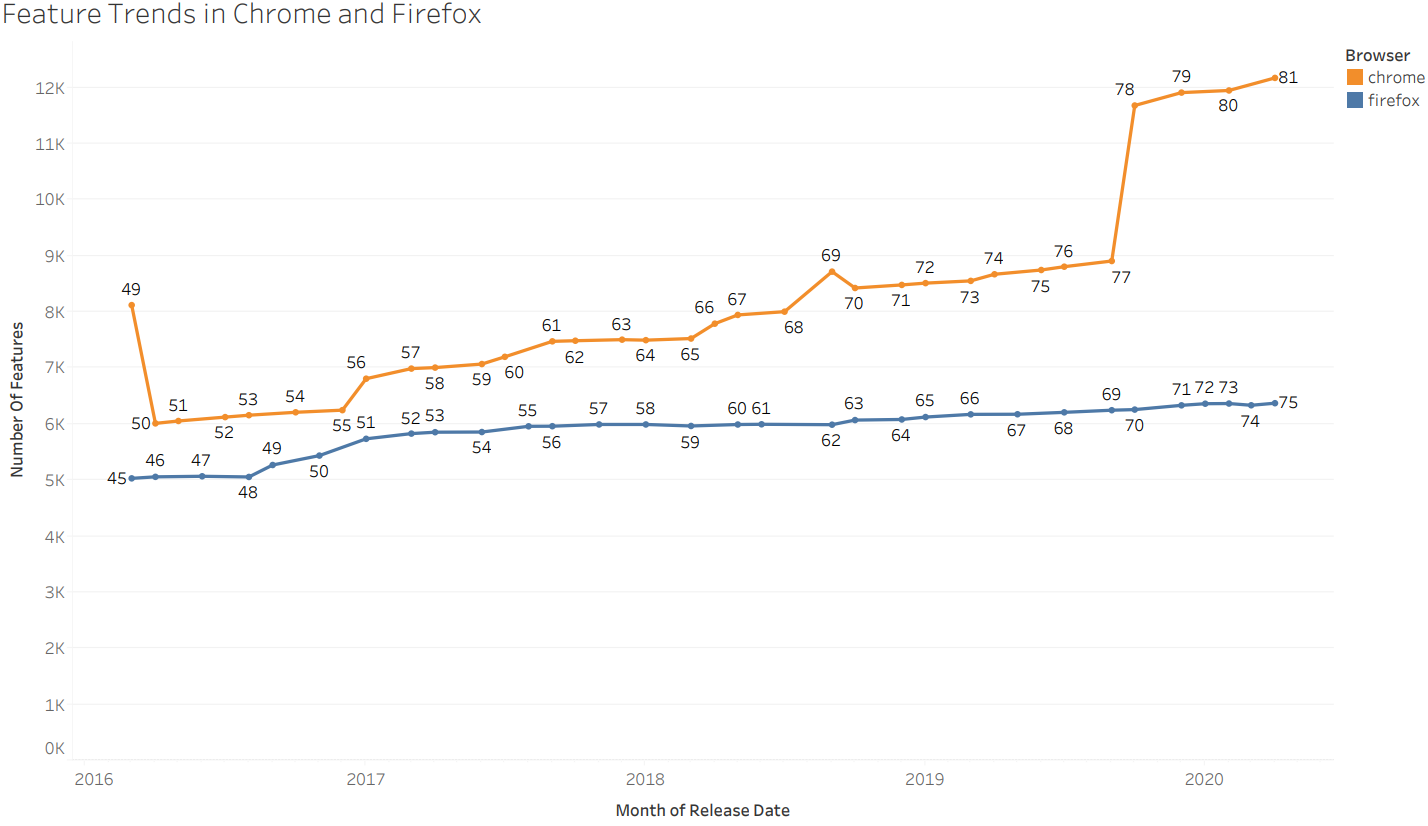
\includegraphics[width=\columnwidth]{figures/Feature-Trends.PNG}
    \caption{Feature trends in Firefox and chrome. The blue line represents the number of features in chrome. The yellow line represents Firefox.\ali{Need to re-scale the chart so the text could be visible}}
    \label{fig:times_bar}
\end{figure}
